\numberedchapter{Additional results}\label{chaper:results}

\begin{figure}[ht]
    \centering
    \captionsetup[subfigure]{justification=centering}
    \begin{subfigure}[h]{0.32\textwidth}
        \centering
        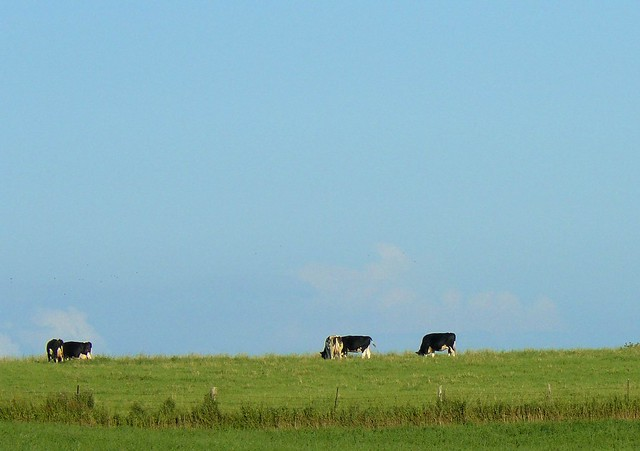
\includegraphics[width=\textwidth]{results/inpaint3.png}
        \caption{Original image}
        \label{fig:original3}
    \end{subfigure}
    \hspace*{\fill}
    \begin{subfigure}[h]{0.32\textwidth}
        \centering
        
\includegraphics[width=\textwidth]{results/mask3.png}
        \caption{Inpainting mask}
        \label{fig:mask3}
    \end{subfigure}
    \hspace*{\fill}
    \begin{subfigure}[h]{0.32\textwidth}
        \centering
        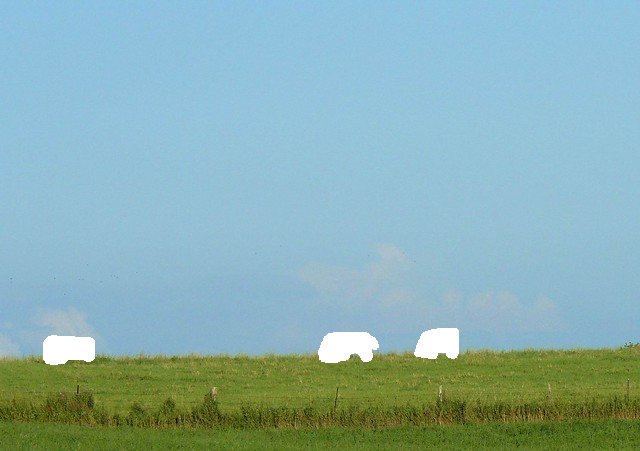
\includegraphics[width=\textwidth]{results/masked3.png}
        \caption{Masked image}
        \label{fig:masked3}
    \end{subfigure}

    \vskip\baselineskip

    \begin{subfigure}[h]{0.32\textwidth}
        \centering
        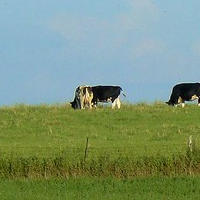
\includegraphics[width=0.46\textwidth]{results/patch3_inpaint2.png}
        \hspace*{0.5mm}
        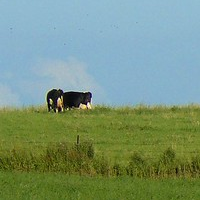
\includegraphics[width=0.46\textwidth]{results/patch3_inpaint.png}
        \caption{Original image - Patches}
        \label{fig:original-patch3}
    \end{subfigure}
    \hspace*{\fill}
    \begin{subfigure}[h]{0.32\textwidth}
        \centering
        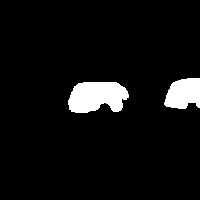
\includegraphics[width=0.46\textwidth]{results/patch3_mask2.png}
        \hspace*{0.5mm}
        
\includegraphics[width=0.46\textwidth]{results/patch3_mask.png}
        \caption{Inpainting mask - Patches}
        \label{fig:mask-patch3}
    \end{subfigure}
    \hspace*{\fill}
    \begin{subfigure}[h]{0.32\textwidth}
        \centering
        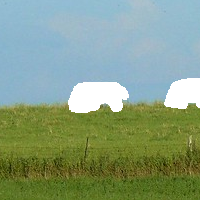
\includegraphics[width=0.46\textwidth]{results/patch3_masked2.png}
        \hspace*{0.5mm}
        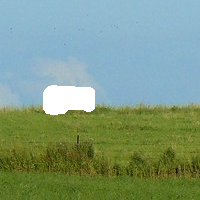
\includegraphics[width=0.46\textwidth]{results/patch3_masked.png}
        \caption{Masked image - Patches}
        \label{fig:masked-patch3}
    \end{subfigure}

    \caption{Masking for an image with inpainting applied at a transition patch}
    \label{fig:masking3}
\end{figure}

\begin{figure}[ht]
    \centering
    \captionsetup[subfigure]{justification=centering}
    \begin{subfigure}[h]{0.32\textwidth}
        \centering
        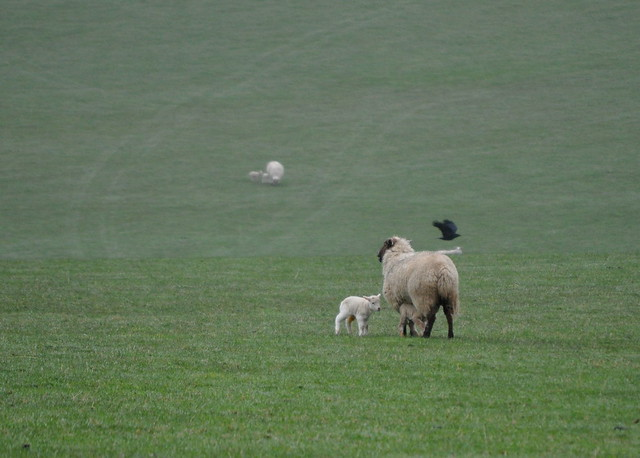
\includegraphics[width=\textwidth]{results/inpaint4.png}
        \caption{Original image}
        \label{fig:original4}
    \end{subfigure}
    \hspace*{\fill}
    \begin{subfigure}[h]{0.32\textwidth}
        \centering
        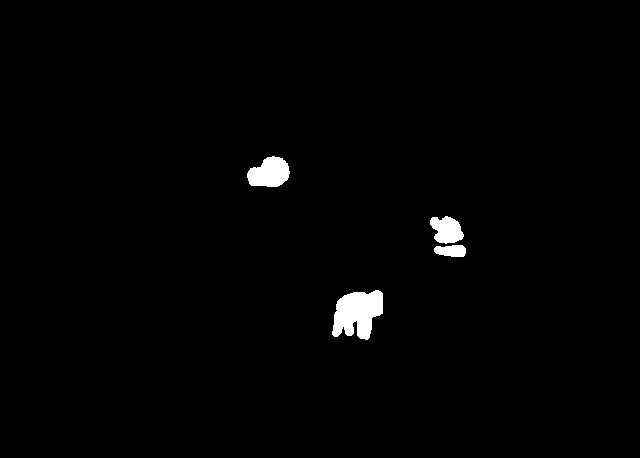
\includegraphics[width=\textwidth]{results/mask4.png}
        \caption{Inpainting mask}
        \label{fig:mask4}
    \end{subfigure}
    \hspace*{\fill}
    \begin{subfigure}[h]{0.32\textwidth}
        \centering
        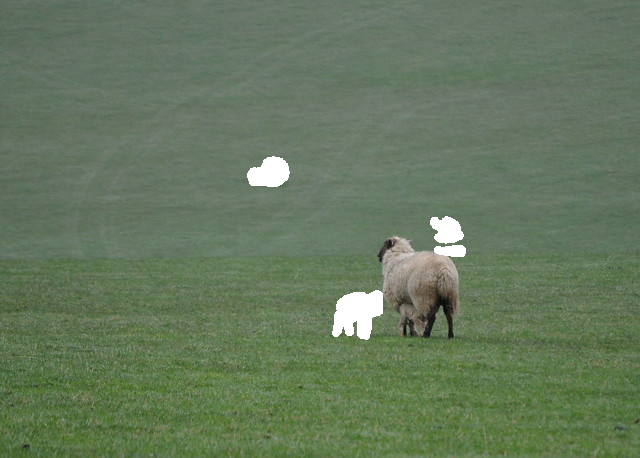
\includegraphics[width=\textwidth]{results/masked4.png}
        \caption{Masked image}
        \label{fig:masked4}
    \end{subfigure}

    \vskip\baselineskip

    \begin{subfigure}[h]{0.32\textwidth}
        \centering
        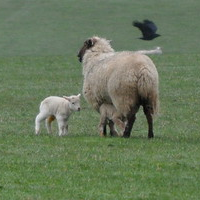
\includegraphics[width=0.46\textwidth]{results/patch4_inpaint2.png}
        \hspace*{0.5mm}
        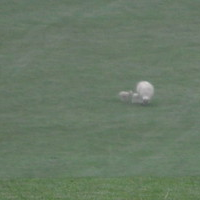
\includegraphics[width=0.46\textwidth]{results/patch4_inpaint.png}
        \caption{Original image - Patches}
        \label{fig:original-patch4}
    \end{subfigure}
    \hspace*{\fill}
    \begin{subfigure}[h]{0.32\textwidth}
        \centering
        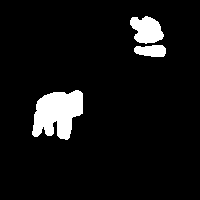
\includegraphics[width=0.46\textwidth]{results/patch4_mask2.png}
        \hspace*{0.5mm}
        
\includegraphics[width=0.46\textwidth]{results/patch4_mask.png}
        \caption{Inpainting mask - Patches}
        \label{fig:mask-patch4}
    \end{subfigure}
    \hspace*{\fill}
    \begin{subfigure}[h]{0.32\textwidth}
        \centering
        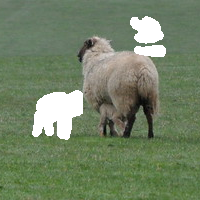
\includegraphics[width=0.46\textwidth]{results/patch4_masked2.png}
        \hspace*{0.5mm}
        
\includegraphics[width=0.46\textwidth]{results/patch4_masked.png}
        \caption{Masked image - Patches}
        \label{fig:masked-patch4}
    \end{subfigure}

    \caption{Masking for an image with inpainting applied on a non-uniform local patch}
    \label{fig:masking4}
\end{figure}

\begin{figure}[ht]
    \centering
    \captionsetup[subfigure]{justification=centering}
    \begin{subfigure}[h]{0.49\textwidth}
        \centering
        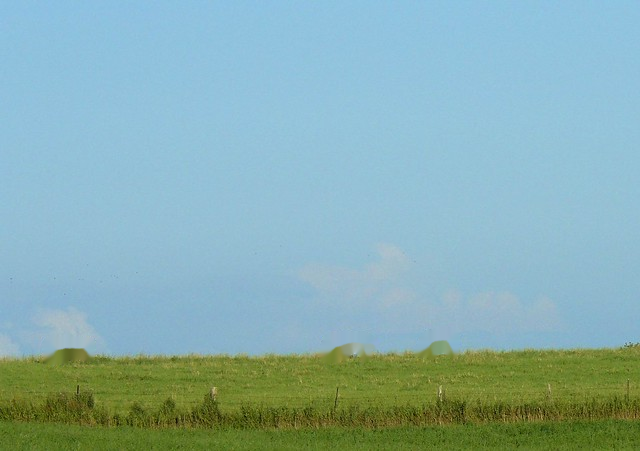
\includegraphics[width=\textwidth]{results/ns3.png}
        \caption{Navier-Stokes}
        \label{fig:ns3}
    \end{subfigure}
    \hspace*{\fill}
    \begin{subfigure}[h]{0.49\textwidth}
        \centering
        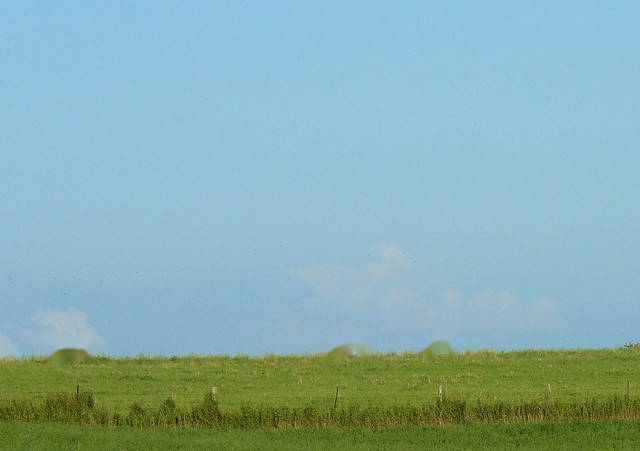
\includegraphics[width=\textwidth]{results/telea3.png}
        \caption{Telea}
        \label{fig:telea3}
    \end{subfigure}

    \vskip\baselineskip

    \begin{subfigure}[h]{0.49\textwidth}
        \centering
        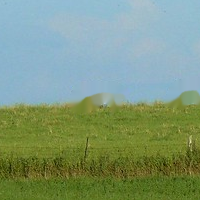
\includegraphics[width=0.46\textwidth]{results/patch3_ns2.png}
        \hspace*{0.5mm}
        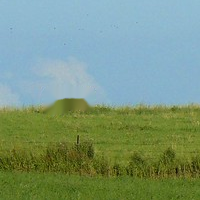
\includegraphics[width=0.46\textwidth]{results/patch3_ns.png}
        \caption{Navier-Stokes - Patches}
        \label{fig:ns-patch3}
    \end{subfigure}
    \hspace*{\fill}
    \begin{subfigure}[h]{0.49\textwidth}
        \centering
        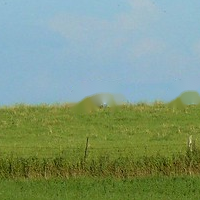
\includegraphics[width=0.46\textwidth]{results/patch3_telea2.png}
        \hspace*{0.5mm}
        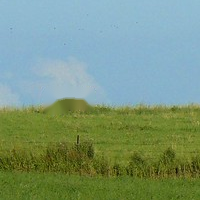
\includegraphics[width=0.46\textwidth]{results/patch3_telea.png}
        \caption{Telea - Patches}
        \label{fig:telea-patch3}
    \end{subfigure}

    \vskip\baselineskip

    \begin{subfigure}[h]{0.49\textwidth}
        \centering
        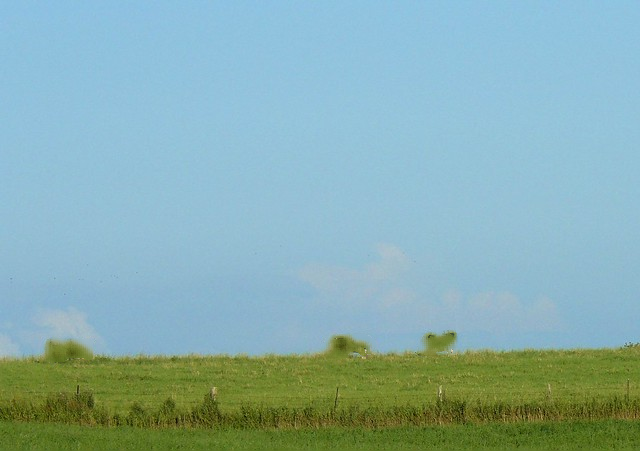
\includegraphics[width=\textwidth]{results/pm3.png}
        \caption{PatchMatch}
        \label{fig:pm3}
    \end{subfigure}
    \hspace*{\fill}
    \begin{subfigure}[h]{0.49\textwidth}
        \centering
        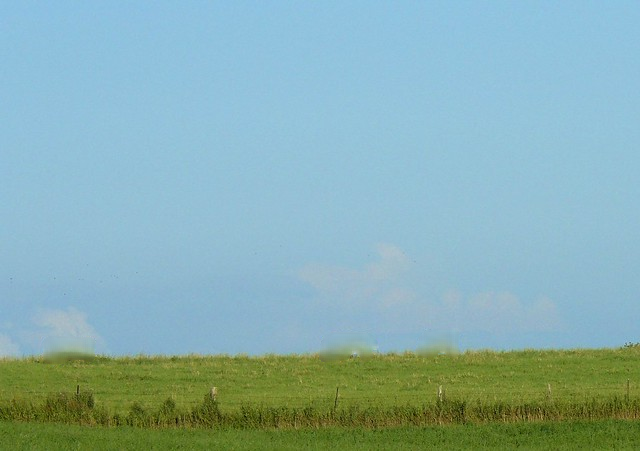
\includegraphics[width=\textwidth]{results/result3.png}
        \caption{GatedResNet}
        \label{fig:inpainted3}
    \end{subfigure}

    \vskip\baselineskip

    \begin{subfigure}[h]{0.49\textwidth}
        \centering
        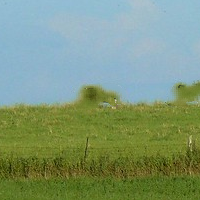
\includegraphics[width=0.46\textwidth]{results/patch3_pm2.png}
        \hspace*{0.5mm}
        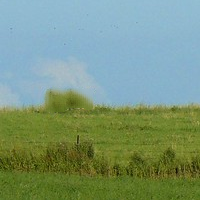
\includegraphics[width=0.46\textwidth]{results/patch3_pm.png}
        \caption{PatchMatch - Patches}
        \label{fig:pm-patch3}
    \end{subfigure}
    \hspace*{\fill}
    \begin{subfigure}[h]{0.49\textwidth}
        \centering
        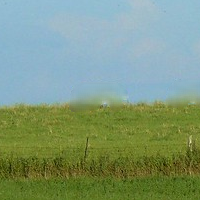
\includegraphics[width=0.46\textwidth]{figures/results/patch3_result2.png}
        \hspace*{0.5mm}
        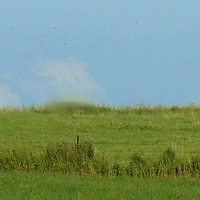
\includegraphics[width=0.46\textwidth]{figures/results/patch3_result.png}
        \caption{GatedResNet - Patches}
        \label{fig:inpainted-patch3}
    \end{subfigure}

    \caption{Comparison for an image with inpainting applied at a transition patch}
    \label{fig:inpainting3}
\end{figure}

\begin{figure}[ht]
    \centering
    \captionsetup[subfigure]{justification=centering}
    \begin{subfigure}[h]{0.49\textwidth}
        \centering
        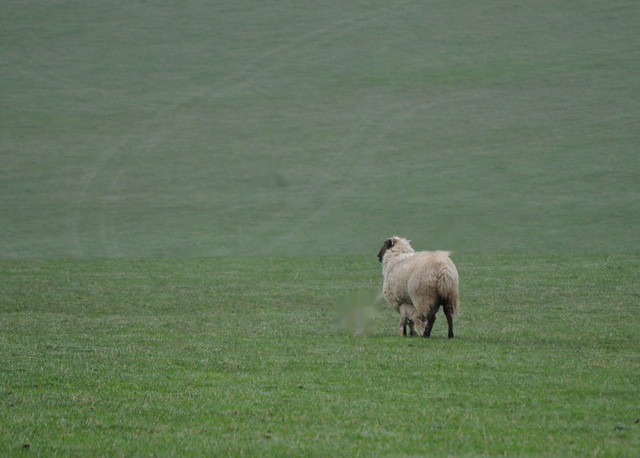
\includegraphics[width=\textwidth]{results/ns4.png}
        \caption{Navier-Stokes}
        \label{fig:ns4}
    \end{subfigure}
    \hspace*{\fill}
    \begin{subfigure}[h]{0.49\textwidth}
        \centering
        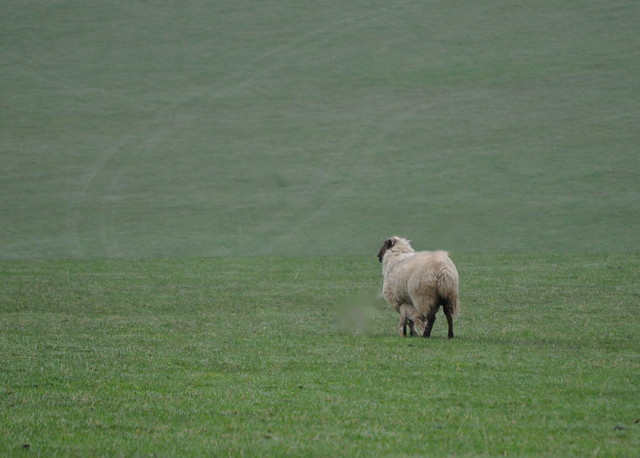
\includegraphics[width=\textwidth]{results/telea4.png}
        \caption{Telea}
        \label{fig:telea4}
    \end{subfigure}

    \vskip\baselineskip

    \begin{subfigure}[h]{0.49\textwidth}
        \centering
        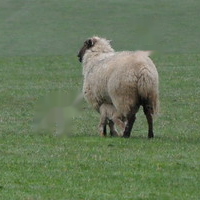
\includegraphics[width=0.46\textwidth]{results/patch4_ns2.png}
        \hspace*{0.5mm}
        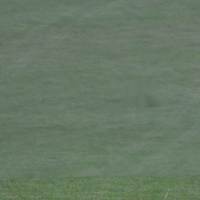
\includegraphics[width=0.46\textwidth]{results/patch4_ns.png}
        \caption{Navier-Stokes - Patches}
        \label{fig:ns-patch4}
    \end{subfigure}
    \hspace*{\fill}
    \begin{subfigure}[h]{0.49\textwidth}
        \centering
        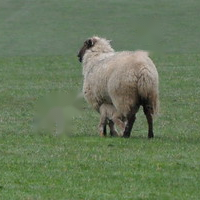
\includegraphics[width=0.46\textwidth]{results/patch4_telea2.png}
        \hspace*{0.5mm}
        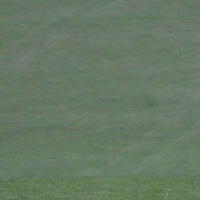
\includegraphics[width=0.46\textwidth]{results/patch4_telea.png}
        \caption{Telea - Patches}
        \label{fig:telea-patch4}
    \end{subfigure}

    \vskip\baselineskip

    \begin{subfigure}[h]{0.49\textwidth}
        \centering
        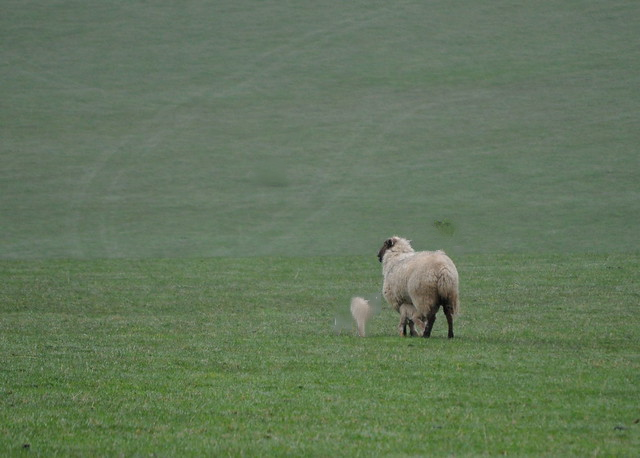
\includegraphics[width=\textwidth]{results/pm4.png}
        \caption{PatchMatch}
        \label{fig:pm4}
    \end{subfigure}
    \hspace*{\fill}
    \begin{subfigure}[h]{0.49\textwidth}
        \centering
        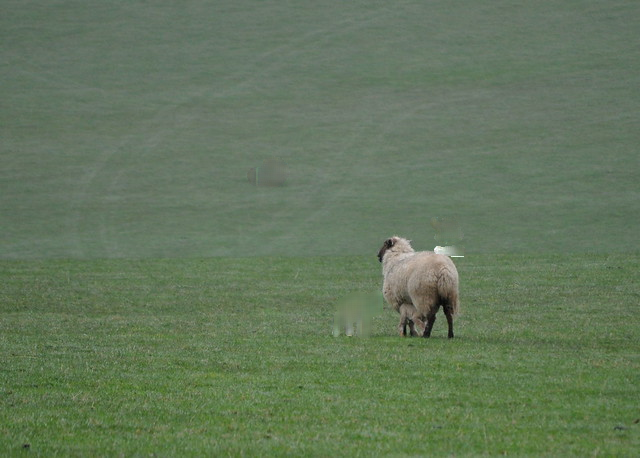
\includegraphics[width=\textwidth]{results/result4.png}
        \caption{GatedResNet}
        \label{fig:inpainted4}
    \end{subfigure}

    \vskip\baselineskip

    \begin{subfigure}[h]{0.49\textwidth}
        \centering
        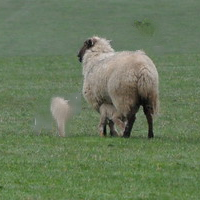
\includegraphics[width=0.46\textwidth]{results/patch4_pm2.png}
        \hspace*{0.5mm}
        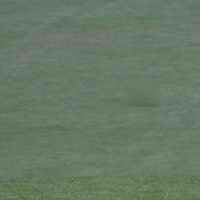
\includegraphics[width=0.46\textwidth]{results/patch4_pm.png}
        \caption{PatchMatch - Patches}
        \label{fig:pm-patch4}
    \end{subfigure}
    \hspace*{\fill}
    \begin{subfigure}[h]{0.49\textwidth}
        \centering
        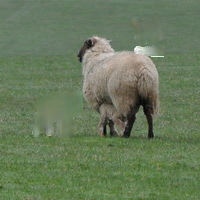
\includegraphics[width=0.46\textwidth]{results/patch4_result2.png}
        \hspace*{0.5mm}
        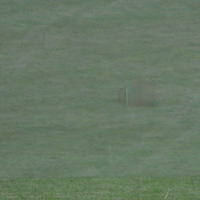
\includegraphics[width=0.46\textwidth]{results/patch4_result.png}
        \caption{GatedResNet - Patches}
        \label{fig:inpainted-patch4}
    \end{subfigure}

    \caption{Comparison for an image with inpainting applied on a non-uniform local patch}
    \label{fig:inpainting4}
\end{figure}
